\chapter{Whole-Body Control of Humanoid Robots with Link Flexibility\label{chapter:flexible_joints}}

In Chapter~\ref{chapter:benchmarking_wbc}, we presented a whole-body controller for humanoid robots in contact with a rigid environment. We then extended the controller in the case of visco-elastic walking surface -- Chapter~\ref{chapter:wbc_visco_elastic}. However, both architectures assume that the links of the robot do not deform during the locomotion task. This hypothesis is generally valid; however, it may happen that one of the links of the system flexes while walking. In this chapter, we attempt to loosen the rigid body hypothesis that has been considered in Chapters~\ref{chapter:benchmarking_wbc} and \ref{chapter:wbc_visco_elastic}. More specifically, we extend the whole-body controller introduced in Section~\ref{sec:dynamics_QP} in the case of a humanoid robot affected by undesired link flexibility.
\par
We characterize the link flexibility by introducing equivalent passive joints where the link
deflection is concentrated~\citep{Nakaoka2007Constraint-basedMechanisms}. We extend the robot state to consider the
underactuated flexible joints in the model. Thanks to this choice, we are able to design a
whole-body controller that implicitly considers the deformation of the joints.
Since in our case the deflection is not directly measurable, we design an observer aiming at
estimating the flexible joint state, namely position, velocity, and torque, only considering the
measured contact force and the actuated joint state.
We validate the overall approach on a simulated version of the humanoid robot TALOS, since its hip
flexibility has a significant impact when performing a locomotion
task~\citep{Villa2022TorqueFlexibility}. To address the elasticity of the robot link, the authors of
\citep{Villa2022TorqueFlexibility} locally compensate the effect of deflections by modifying the
measured position and velocity of some actuated joints considered in the whole-body controller. By
extending the robot state with passive joints, our approach automatically considers the link
flexibility in the control stabilization problem.
\par
To further test the proposed strategy, we compare the whole-body control presented in this chapter with the approach discussed in Section~\ref{sec:dynamics_QP}. In this respect, we investigate the flexibility of the link that makes classical approaches fail. Finally, we analyze the performance of the presented control design with respect to different values of the stiffness parameter.
\par
The chapter is organized as follows. Section~\ref{sec:flex_joint_system_modeling} details the model used to characterize the flexibility of the link and extends the humanoid robot model to account for it. Section~\ref{sec:wbc_tsid_flex_joints} discusses the whole-body controller. Section~\ref{sec:flexible_joint_observer} contains the design of an observer to estimate the flexible joint state online. Section~\ref{sec:flexible_joint_result} presents the simulation results on the TALOS humanoid robot. Finally, Section~\ref{sec:conclusions_flexible_joint} concludes the chapter.
The content of this chapter has been carried out during my Ph.D. secondment in the \emph{Gepetto} laboratory of the \emph{LAAS-CNRS Laboratory for Analysis and Architecture of Systems} in Toulouse, France.
The control architecture presented in this chapter is the subject of a publication to be submitted:
\fcite{Romualdi2022ControlControl}

\section{System modeling\label{sec:flex_joint_system_modeling}}

TALOS's hip flexibility has a significant impact on its leg control and, as a result, its balance and locomotion~\citep{Ramuzat2021ComparisonTALOS}. In this section, we model the TALOS's hip flexibility by means of underactuated joints. The section also extends the humanoid robot model dynamics presented in Section~\ref{sec:multi-body-dynamics} to consider the robot's link visco-elasticity.

\subsection{Model of the hip flexibility}

Following the work of~\cite{Villa2022TorqueFlexibility}, we model the flexibility by introducing two passive virtual joints between the base link and each leg. The virtual joints simulate the motion caused by the visco-elastic deformation of the waist-leg connection, where the link cross section is reduced.
Given the $i$-th passive joint, we assume that it exerts a torque $\tau^f_i$ that depends on the
joint deflection $s^f_i$ and its velocity $\dot{s}^f_i$~\citep{Nakaoka2007Constraint-basedMechanisms} as
\begin{equation}
\label{eq:flexible_joint}
\tau^f_i = -k_i s^f_i - d_i \dot{s}^f_i.
\end{equation}
where $k_i$ and $d_i$ are, respectively, the stiffness and damping coefficients of the flexible
joint $i$. By assuming to model the link flexibility with $n_f$ joints, we can consider the robot to
have $n$ joints where $n = n_a + n_f$ with $n_a$ are the actuated joints.
\par
In the specific case of the TALOS robot, the authors of \citep{Villa2022TorqueFlexibility} notice that
the stiffness is due to the vertical linkage and, consequently, they model the flexibility along
the pitch and roll axis, only. In this chapter, the same consideration holds, so we introduce two
passive flexible joints for each leg. As a result $n_f = 4$ while $n_a = 32$ -- see Section~\ref{sec:talos}.
\par
Assuming that it is possible to estimate $\tau^f_i$, we approximate the flexible joint state by discretizing
Equation~\eqref{eq:flexible_joint}, resulting in
\begin{IEEEeqnarray}{C}
\phantomsection \label{eq:flexibility_discretized} \IEEEyesnumber \IEEEyessubnumber*
s^f_i[k] = \frac{d_i s^f_i[k-1] - \tau^f_i[k] \diff t}{k_i \diff t + d_i}, \label{eq:flexibility_discretized_position} \\
\dot{s}^f_i[k] = \frac{s^f_i[k] - s^f_i[k-1]}{\diff t}.
\end{IEEEeqnarray}
Here $\diff t$ is the sampling time. $s^f_i[k] = s^f_i(t_0 + k \diff t)$ and $\dot{s}^f_i[k] = \dot{s}^f_i(t_0 + k \diff t)$.


\subsection{Modeling of a floating base system with flexible joints}
This section extends the floating base system model presented in Section~\ref{sec:multi-body-dynamics} to consider underactuated flexible joints.
\par
Let us consider an inertial frame $\mathcal{I}$ and a floating base system making $n_c$ contact with the environment. We recall:
\begin{itemize}
    \item $B = (p_B, [B])$ is the frame rigidly attached to the robot base. ${}^\mathcal{I} H _B \in \SE(3)$  describes the position and orientation of $B$ with respect to the inertial frame $\mathcal{I}$.
    \item Hereafter the base velocity expressed in mixed representation ${}^{B[\mathcal{I}]}\mathrm{v}_{\mathcal{I}, B}$ such that  ${}^{B[\mathcal{I}]}\mathrm{v}_{\mathcal{I}, B}^\top = \begin{bmatrix}
    {}^{\mathcal{I}} \dot{p}_B^\top & {}^{B[\mathcal{I}]}\dot{\omega}_{\mathcal{I}, B}^\top.
    \end{bmatrix}$
    \item The actuated and flexible joint positions are indicated, respectively, with $s^a \in \mathbb{R}^{n_a}$ and $s^f \in \mathbb{R}^{n_f}$;
    \item the actuated and flexible joint torques are indicated, respectively, with $\tau^a \in \mathbb{R}^{n_a}$ and $\tau^f \in \mathbb{R}^{n_f}$.
\end{itemize}
We extend the robot configuration~\eqref{eq:robot_configuration_mixed} by introducing the flexible
joint value as $q = ({}^{\mathcal{I}} p_B, {}^{\mathcal{I}} R_{B}, s^a, s^f)$. $q$ is an element
of a Lie group $\lieGroup{Q} = \mathbb{R}^3 \times SO{(3)} \times \mathbb{R}^{n_a} \times
\mathbb{R}^{n_f}$. The associated lie Algebra writes as $\lieAlgebra{q} = \mathbb{R}^3 \times \so(3)
\times \mathbb{R}^{n_a} \times \mathbb{R}^{n_f}$. Here, we recall that $\lieAlgebra{q}$ is isomorphic to $\mathbb{R}^3 \times \mathbb{R}^3 \times \mathbb{R}^{n_a} \times \mathbb{R}^{n_f}$ -- see Appendix~\ref{sec:tangent_space_lie}.
\par
The \emph{velocity of the multi-body system} belongs to $\lieAlgebra{q}$ and we denote it with $\nu = \left({}^{\mathcal{I}} \dot{p}_B, {}^{B[\mathcal{I}]}{\omega}_{\mathcal{I}, B}, \dot{s}^a, \dot{s}^f\right)$.
\par
Slightly modifying~\eqref{eq:system}, we write the dynamics of a floating base system with flexible joints as follows 
\begin{equation}
\label{eq:system_flex}
{M}({q})\dot{{\nu}} + h({q}, {\nu}) =  \begin{bmatrix}
{0}_{6\times n_a} \\ I_{n_a} \\ 0_{n_f\times n_a}
\end{bmatrix}{\tau}^a + 
\begin{bmatrix}
{0}_{6\times n_f} \\ 0_{n_a\times n_f} \\ I_{n_f} 
\end{bmatrix}{\tau}^f +
             {J}_{\mathcal{C}}(q)^\top \mathrm{f},
\end{equation}
where
\begin{equation}
	{J}_{\mathcal{C}}({q}) = 
	\begin{bmatrix}{J}_{\mathcal{C}_1}({q}) \\ \vdots \\ {J}_{\mathcal{C}_{n_c}}({q})  \end{bmatrix}, \quad
	\mathrm{f} = \begin{bmatrix}
		{}_{\mathcal{C}_1[\mathcal{I}]}\mathrm{f}_1 \\
		\vdots\\
		{}_{\mathcal{C}_{n_c}[\mathcal{I}]}\mathrm{f}_{n_c}
	\end{bmatrix}.
\end{equation}
Recalling that $n=n_a + n_f$, $M\in \mathbb{R}^{(n+6) \times (n+6)}$ is the mass matrix,
$h \in \mathbb{R}^{(n+6)}$ accounts for Coriolis, the centrifugal effects and the gravity term.  ${}_{\mathcal{C}_k[\mathcal{I}]}\mathrm{f}_k \in \mathbb{R}^{6}$ denotes the $k$-th external wrench applied by the environment on the robot expressed in mixed representation.
The Jacobian $J_{\mathcal{C}_k}$ is the mixed velocity Jacobian of the contact $\mathcal{C}_k$.
\par
Following the same approach presented in Section~\ref{sec:multi-body-dynamics}, the
dynamics~\eqref{eq:system_flex} is expressed by separating the first $6$ rows, which refers to the underactuated floating base, from the last rows $n_a + n_f$, which refers to the actuated and flexible joints as:
\begin{IEEEeqnarray}{c}
\IEEEyesnumber \phantomsection
M_{\nu}(q) \dot{\nu} + h_{\nu} (q, \nu) =  J^\top_{{\mathcal{C}}_\nu}(q) \;  \mathrm{f},\label{eq:system_flex_base_projection} \IEEEyessubnumber \\
M_{s}(q) \dot{\nu} + h_{s} (q, \nu) = \begin{bmatrix}
I_{n_a} \\ 0_{n_f\times n_a}
\end{bmatrix}{\tau}^a +
\begin{bmatrix}
 0_{n_a\times n_f} \\ I_{n_f}
\end{bmatrix}{\tau}^f +  J^\top_{{\mathcal{C}}_s}(q)  \; \mathrm{f}. \label{eq:system_flex_joint_projection} \IEEEyessubnumber
\end{IEEEeqnarray}
The subscript $\nu$ refers to the first $6$ rows of the matrix, while $s$ refers to the last $n$
rows. Equation~\eqref{eq:system_flex_base_projection} is often denoted as the base projection of the floating base dynamics, while
Equation~\eqref{eq:system_flex_joint_projection} is the joint space projection.

\section{Whole-body Controller\label{sec:wbc_tsid_flex_joints}}
Similar to what is discussed in Sections~\ref{sec:dynamics_QP} and \ref{sec:controller_tsid_compliant},
the goal of the whole-body controller is to guarantee the tracking of desired kinematic quantities while ensuring the feasibility of the contact forces.
In this section, we present an extension of the dynamics-based whole-body controller of Section
\ref{sec:dynamics_QP} that considers the floating base dynamics in the case of under-actuated flexible joints -- Equation~\eqref{eq:system_flex}.
\par
The proposed controller computes the desired robot actuated joint torques $\tau^a$, the generalized
acceleration ${}^{B[\mathcal{I}]}\dot{\nu}$, and a set of desired spatial contact forces expressed
in mixed representation ${}_{\mathcal{C}_j[\mathcal{I}]}\mathrm{f}_j$. Following the same approach
as in Section~\ref{sec:dynamics_QP}, we formulate the control problem using the stack of tasks
approach. We transcribe the optimal control problem into a constrained optimization problem. Here, we
consider the low priority tasks as the terms of the cost function, while the high priority tasks are modeled as constraints.

\subsection{Low and high priority tasks}
This section introduces the list of low and high priority tasks considered in the optimal control problem.

\subsubsection{Centroidal momentum task}
Given a frame $\bar{G} = (x_\text{CoM},[\mathcal{I}])$, we introduce the centroidal momentum task as in Section~\ref{sec:tsid_tasks}:
\begin{equation}
    \label{eq:tsid_centroidal_momentum_joint_flex}
    \Psi_h = {}_{\bar{G}} \dot{{h}}^* - A_c \mathrm{f} - m\bar{g}.
\end{equation}
where $m$ is the robot mass, $\bar{g} = \begin{bmatrix} 0&0&-g&0&0&0 \end{bmatrix}^\top$ is the 6D gravity acceleration. $A_c$ is the matrix containing the co-adjoint transformations ${}_{\bar{G}} X^{\mathcal{C}_i[\mathcal{I}]}$, i.e.
\begin{equation}
    A_c = \begin{bmatrix}
    {}_{\bar{G}} X ^{\mathcal{C}_1[\mathcal{I}]} & \hdots & {}_{\bar{G}} X^{\mathcal{C}_{n_c}[\mathcal{I}]}.
    \end{bmatrix}
\end{equation}
${}_{\bar{G}} \dot{{h}}^*$ is chosen considering~\eqref{eq:tsid_h_p_star} and \eqref{eq:tsid_h_omega_star} as:
\begin{equation}
    \label{eq:tsid_h_star_flex_joints}
    {}_{\bar{G}} \dot{{h}}^* = 
    \begin{bmatrix}
    m  \ddot{x}^\text{ref}_\text{CoM} \\ 
    {}_{\bar{G}} \dot{{h}}^{\omega^\text{ref}} 
    \end{bmatrix} +
    \begin{bmatrix}
    m K^d_\text{CoM}& 0_{3\times3}\\
     0_{3\times3} & K_{h^\omega}
    \end{bmatrix}
    \begin{bmatrix}
    \dot{x}^\text{ref}_\text{CoM} - \dot{x}_\text{CoM} \\ 
    {}_{\bar{G}} {{h}}^{\omega^\text{ref}} - {}_{\bar{G}} {{h}}^{\omega}
\end{bmatrix} 
 +
    \begin{bmatrix}
    m K^p_\text{CoM} \\
     0_{3\times3} 
    \end{bmatrix}
\left({x}^\text{ref}_\text{CoM} - {x}_\text{CoM}\right).
\end{equation}
In our scenario, the desired centroidal quantities ${x}^\text{ref}_\text{CoM}$ and ${}_{\bar{G}} {{h}}^{\omega}$ are provided by a high-level planner.

\subsubsection{Cartesian task}
Similar to what was discussed in Section~\ref{sec:tsid_tasks}, the Cartesian task is implemented as:
\begin{equation}
\label{eq:tsid_se3_task_flex_joint}
    \Psi_{L_{\SE(3)}} =  {}^{L[\mathcal{I}]}\dot{\mathrm{v}}_{\mathcal{I},L}^* - J_{L} \dot{\nu} - \dot{J}_{L} {\nu}
\end{equation}
where $ {}^{L[\mathcal{I}]}\dot{\mathrm{v}}^*_{\mathcal{I},L} =\begin{bmatrix}
\ddot{p}_L^{*^\top} & {}^\mathcal{I}\dot{\omega}^{*^\top}_{\mathcal{I},L}
\end{bmatrix} ^\top $ is chosen as~\eqref{eq:tsid_se3_task_velocity}.
Similarly, we recall that the positional and rotational tasks are given by
Equations~\eqref{eq:tsid_r3_task} and \eqref{eq:tsid_so3_task}.
As we discuss in more depth in Section~\ref{sec:joint_flex_optimal_control}, we apply this task
to stabilize the orientation of the chest and the root and the pose of the feet.

\subsubsection{Floating base dynamics task}
If the robot is equipped with under-actuated flexible joints, the whole-body controller should consider the measured (or estimated) joint torques acting on the flexibility. To do so, we modify the floating base dynamics task presented in Section~\ref{sec:tsid_tasks}. 
We project the dynamics~\eqref{eq:system_flex} into the base and joint subspaces, and we name the projection as \emph{base dynamics} and \emph{joint dynamics} -- see Section~\ref{sec:multi-body-dynamics}. We define the base dynamics constraint as~\eqref{eq:tsid_base_dyn_task}
\begin{equation}
    \label{eq:tsid_base_dyn_task_flex_joint}
    \Psi_{\text{dyn}_\nu} =  h_{\nu} +  M_{\nu}\dot{\nu} - J_{\mathcal{C}_\nu}^\top \mathrm{f}.
\end{equation}
Equation~\eqref{eq:tsid_base_dyn_task_flex_joint} does not depend on the flexible joint state.
The joint dynamics task is given by
\begin{equation}
    \label{eq:tsid_joint_dyn_task_flex_joint}
    \Psi_{\text{dyn}_s} =  h_{s} +  M_{s}(q) \dot{\nu} - \begin{bmatrix}
    I_{n_a} \\
    0_{n_f \times n_a}
    \end{bmatrix}
    \tau^a -
    \begin{bmatrix}
    0_{n_a \times n_f} \\
    I_{n_f}
    \end{bmatrix}
    \tau^f - J_{\mathcal{C}_s}^\top \mathrm{f}.
\end{equation}
The subscript $\nu$ refers to the first six rows of the matrix, while $s$ refers to the last $n_a + n_f$ rows. 
We notice that the last $n_f$ rows of \eqref{eq:tsid_joint_dyn_task_flex_joint} represent the underactuated dynamics due to joint flexibility.

\subsubsection{Joint position regularization task}
To prevent the controller from computing solutions that generate a huge variation in joint acceleration, we introduce a joint regularization task for both the actuated and flexible joints, as
\begin{IEEEeqnarray}{C}
\phantomsection \label{eq:tsid_s_task_join_flex} \IEEEyesnumber \IEEEyessubnumber* 
\Psi_{s_a} = \ddot{s}^*_a - \begin{bmatrix}
    0_{n_a\times6} & I_{n_a} & 0_{n_a \times n_f} 
    \end{bmatrix} \dot{\nu} \label{eq:tsid_s_task_join_flex_actuated} \\
\Psi_{s_f} = \ddot{s}^*_f - \begin{bmatrix}
    0_{n_f\times6}  & 0_{n_f \times n_a} & I_{n_f}
    \end{bmatrix} \dot{\nu} \label{eq:tsid_s_task_join_flex_flex},
\end{IEEEeqnarray}
with $\ddot{s}^*_a$ is equal to
\begin{equation}
    \ddot{s}^*_a = \ddot{s}^\text{ref}_a + k_{s_a}^d (\dot{s}^\text{ref}_a - \dot{s}_a) + k_{s_a}^p (s^\text{ref}_a - s_a).
\end{equation}
where $s^\text{ref}_a$ is the desired joint trajectory provided by a high-level planner. $k_{s_a}^d$
and $k_{s_a}^p$ are two positive-defined diagonal matrices.
On the other hand, assuming that we estimate the state of the flexible joints, we ask for $\ddot{s}^*_f$ equal to
\begin{equation}
  \label{eq:flex_joint_position_regularization_flex}
    \ddot{s}^*_f = - k_{s_f}^d \dot{s}_f - k_{s_f}^p  s_f.
\end{equation}
where $k_{s_f}^d$ and $k_{s_f}^p$ are two defined positive diagonal matrices. Thanks
to~\eqref{eq:flex_joint_position_regularization_flex} the controller tries to stabilize the flexible
joint position to zero.

\subsubsection{Joint torque regularization task}
In order to prevent the controller from providing solutions with large actuated joint torques, we introduce the following task:
\begin{equation}
    \label{eq:tsid_tau_regularization_task_flex_joint}
    \Psi_\tau = \tau^\text{ref}_a - \tau_a,
\end{equation}
where, in our case, $\tau^\text{ref}_a$ is provided by a high-level planner.

\subsubsection{Feasibile contact force task}
The feasibility of the contact wrench ${}_{\mathcal{C}_j[\mathcal{I}]}\mathrm{f}_j$ is guaranteed by the set of inequalities introduced in Equation~\eqref{eq:tsid_contact_wrench_feasibility_constraint}:
\begin{equation}
  \Phi_{\mathrm{f}_j}: \;\;  \label{eq:tsid_contact_wrench_feasibility_constraint_flex}
    A_{\mathcal{C}_j[\mathcal{I}]} \; {}_{\mathcal{C}_j[\mathcal{I}]}\mathrm{f}_j - b  \preceq 0.
\end{equation}
we recall that $A_{\mathcal{C}_j[\mathcal{I}]}$ depends on the robot generalized state $q\in \mathcal{Q}$.

\subsection{Quadratic programming problem \label{sec:joint_flex_optimal_control}}
Following the same approach as in Section~\ref{sec:tsid_optimal_control_problem}, we achieve the
control objective by transcribing the control problem as a constrained quadratic programming problem. Here, we consider the contact forces ${}_{\mathcal{C}_j[\mathcal{I}]}\mathrm{f}_j$, the base acceleration ${}^{B[\mathcal{I}]} \dot{\mathrm{v}}_{\mathcal{I}, B}$, the actuated joint acceleration $\ddot{s}_a$, and the actuated joint torques $\tau_a$ as conditional variables.
\par
The tracking of the left and right feet are considered high-priority $\SE(3)$ tasks~\eqref{eq:tsid_se3_task_flex_joint} and they are denoted respectively as $\Psi_{L_{\SE(3)}}$ and $\Psi_{R_{\SE(3)}}$. We take into account the centroidal momentum tracking as a high priority task~\eqref{eq:tsid_centroidal_momentum_joint_flex}. The desired centroidal quantities $x_\text{CoM}^\text{ref}$ and $h_\omega^\text{ref}$ in \eqref{eq:tsid_h_star_flex_joints} are provided by a high-level planner that assumes that all robot joints are fully actuated. We also consider the base~\eqref{eq:tsid_base_dyn_task_flex_joint} and joints dynamics~\eqref{eq:tsid_joint_dyn_task_flex_joint} as high priority tasks. To prevent the controller from asking for a high motion of the upper body while stabilizing the CoM, we introduce two $\SO(3)$ tasks, one associated with the chest and the other with the waist orientations, respectively, denoted $\Psi_{T_{\SO(3)}}$ and $\Psi_{R_{\SO(3)}}$. In both cases, we ask to keep the z coordinates of the link frames parallel to the gravity vector $g$. The postural conditions of the actuated and flexible joints~\eqref{eq:tsid_s_task_join_flex} are considered low priority tasks.  We regularize the desired actuated joint torques as a low priority task $\Psi_\tau$~\eqref{eq:tsid_tau_regularization_task_flex_joint}. Here $\tau^\text{ref}_a$ is provided by a high-level planner. Finally, to guarantee feasible contact forces for the feet, we add the task~\eqref{eq:tsid_contact_wrench_feasibility_constraint_flex}, denoted respectively as $\Phi_{\mathrm{f}_L}$ and $\Phi_{\mathrm{f}_R}$.
\par
The above hierarchical control objectives can be cast into an optimization problem described by the
following formulation:
\begin{IEEEeqnarray}{CL}
\phantomsection \label{eq:tsid_flex_joints_optimization} \IEEEyesnumber \IEEEyessubnumber*
\;\minimize\limits_{{}^{B[\mathcal{I}]}\mathrm{v}_{\mathcal{I},B},\; \ddot{s}_a ,\; \tau_a, \;\mathrm{f}} \; & \Psi_{T_{\SO(3)}}^\top \Lambda_T \Psi_{T_{\SO(3)}} + \Psi_{R_{\SO(3)}}^\top \Lambda_R \Psi_{R_{\SO(3)}} \\
& + \Psi_{s}^\top \Lambda_s \Psi_{s} + \Psi_{\tau}^\top \Lambda_\tau \Psi_{\tau} \label{eq:tsid_flex_joints_optimization_cost} \\
\st & \Psi_{L_{\SE(3)}} = 0  \label{eq:tsid_flex_joints_optimization_costraint_lf} \\
&  \Psi_{R_{\SE(3)}} = 0 \label{eq:tsid_flex_joints_optimization_costraint_rf} \\
& \Psi_{h} = 0 \label{eq:tsid_flex_joints_optimization_costraint_com} \\
& \Psi_{\text{dyn}_\nu} = 0 \label{eq:tsid_flex_joints_optimization_costraint_dyn_base} \\
& \Psi_{\text{dyn}_s} = 0 \label{eq:tsid_flex_joints_optimization_costraint_dyn_s} \\
&\Phi_{\mathrm{f}_L} \\
&\Phi_{\mathrm{f}_R}
\end{IEEEeqnarray}
Following the same considerations as in Sections~\ref{sec:tsid_optimal_control_problem} and~\ref{sec:tsid_flex_optimal_control_problem}, we transcribe the optimization problem~\eqref{eq:tsid_flex_joints_optimization} into a quadratic programming problem (Section~\ref{sec:qp}) and we solve it via an off-the-shelf solver.

\section{Flexible Joint State Observer\label{sec:flexible_joint_observer}}
The optimal control problem presented in Section~\ref{sec:wbc_tsid_flex_joints} assumes the knowledge of the state of the flexible joints, namely position, velocity, and torque.  In a simulated environment, these values are perfectly known. However, in the real scenario, an estimation algorithm is required to compute them.
\par
In this section, we discuss an algorithm that estimates the flexible joint torques, position, and velocity considering the measured contact wrenches that act on the robot soles and the actuated joint state. For simplicity, we present the algorithm considering the flexibility of the TALOS link. Given the symmetry of the robot structure, we analyze the approach only for one leg.
Even if we approach the problem considering the TALOS use case, we want to underline that the
proposed estimation can also be applied to other humanoid robots affected by link flexibility.
\par
For TALOS, we know that each leg is made up of $8$ joints, $2$ of which are flexible and the other $6$ are actuated. Furthermore, we assume that the flexible joints are located near the waist. As discussed in Section~\ref{sec:floating-base-multi-body-system}, we model the floating base multi-body
system as a kinematic three. Figure~\ref{fig:talos_leg_scheme} presents a schematic representation
of the TALOS leg structure. Exploring the three from the waist to the sole, we first visit the flexible joints, and then the actuated joints.
\begin{figure}[t]
    \centering
	\includegraphics{chapter_flexible_joints/figures/leg_scheme.tikz}
	\caption[Schematic representation of the flexible TALOS leg.]{Schematic representation of the flexible TALOS leg. The links are represented by the graphs node, while the joints are the arcs. $L^a_0$ is the robot waist, $L^f_1$ and $L^f_2$ the flexible links, $L^a_i$ and  $s^a_i$ with $1\le i \le6$ are respectively the robot link and the actuated joints}
	\label{fig:talos_leg_scheme}
\end{figure}
From now on, we denote by $L^a_0$ the waist of the robot, while $L^f_1$ and $L^f_2$ are the fictitious flexible links required to connect the flexible joints $s_1^f$ and $s_2^f$. $L^a_i$ and  $s^a_i$ with $1\le i \le6$ are the robot link and the actuated joints, respectively. Figure~\ref{fig:leg_geometric_scheme} presents the geometric model of the flexible robot leg. Each link is associated with a frame attached to the joint connecting the link to its parent. The name of the frame associated with the link coincides with the name of the link. 
\begin{figure}[t]
    \centering
	\includegraphics{chapter_flexible_joints/figures/leg_geometric_scheme.tikz}
	\caption[Geometric model of the flexible TALOS leg.]{Geometric model of the flexible TALOS leg. Each link is associated with a frame attached to the joint connecting the link to its parent. The red frames are associated with the flexible links while the green frames to the robot links.}
	\label{fig:leg_geometric_scheme}
\end{figure}
\par
Given one link of the leg chain, the associated rigid body dynamics is given by \emph{Eurel-Poincaré Equations} (Equation~\eqref{eq:eurel-poincare-equations-lie-se3-force}): 
\begin{equation}
\label{eq:eurel-poincare-equations-lie-se3-force-flex-joints}
     {}_L \mathbb{M} _ L {}^L \dot{\mathrm{v}} _{\lieGroup{I}, L} + {}^L \mathrm{v} _{\lieGroup{I}, L } \times^* {}_L \mathbb{M} _ L {}^L \mathrm{v} _{\lieGroup{I}, L }  = {}_L \mathbb{M} _ L \begin{bmatrix}
      {}^\lieGroup{I} R _ L ^\top g \\ 
      0_{3\times1}
     \end{bmatrix} + \sum_{k=1}^{n_f} {}_L  \mathrm{f}_k.
\end{equation}
where $L$ is the frame associated with the link. ${}_L \mathbb{M} _ L$ is the 6D constant inertial matrix of the link~\eqref{eq:6d_inertial_matrix_body}. ${}^L \mathrm{v} _{\lieGroup{I}, L }$ is the left-trivialized spatial velocity~\eqref{eq:left_trivialized_velocity_definition}. $g$ is the gravity vector. ${}_L\mathrm{f}_k$ is a 6D spatial force acting on the link, and $n_f$ are the forces acting on the link.
We now assume that each link is subject to only two forces. One is exerted by the parent link, and the other is exerted by the child link. Given the chain structure of the leg (Figure~\ref{fig:talos_leg_scheme}), each link has one parent and one child, except for the waist $L^a_0$ and the foot sole $L^a_6$. With an abuse of notation, we consider the environment as the child of the sole. If the foot is in contact with the ground, one of the 6D forces acting on $L_6^a$ is caused by the interaction with the environment. Since TALOS has a force-torque sensor mounted on the ankle, we assume the ground reaction force is measurable. 
\par
We now introduce the \emph{proper sensor acceleration} as~\citep[Section~2.4.4]{Traversaro2017ModellingDynamics}
\begin{equation}
\label{eq:proper_sensor_acceleration_def}
    \alpha _ {\mathcal{I},L}^g := {}^L X_ {L[\mathcal{I}]} {}^{L[\mathcal{I}]} \dot{\mathrm{v}}_ {\mathcal{I},L} - \
    \begin{bmatrix}
     {}^\lieGroup{I} R _ L ^\top g \\ 
      0_{3\times1}
    \end{bmatrix}.
\end{equation}
Where ${}^L X_ {L[\mathcal{I}]}$ is the adjoint matrix, i.e, ${}^L X_ {L[\mathcal{I}]} = \AdM_{{}^L H_ {L[\mathcal{I}]}}$ -- see Equation~\eqref{eq:adjoint_matrix_se3_def}. 
$\alpha _ {\mathcal{I},L}^g$ is the acceleration obtained by an inertial measurement unit (IMU) aligned with $L$. The linear part is the readout of a linear accelerometer, and the angular part is the derivative of the output of a gyroscope.
\par
Combining the proper sensor acceleration~\eqref{eq:proper_sensor_acceleration_def} with \eqref{eq:eurel-poincare-equations-lie-se3-force-flex-joints}, we rewrite the body dynamics as
\begin{equation}
    {} _ L \mathbb{M} _ L \alpha ^ g _ {\mathcal{I},L} + \begin{bmatrix} 
0 _ {3 \times 1} \\ 
{}^L \omega _{\mathcal{I}, L} \end{bmatrix}  \times ^ * {} _ L \mathbb{M} _ L \begin{bmatrix} 
0 _ {3 \times 1} \\ 
{}^L \omega _{\mathcal{I}, L} \end{bmatrix} =   \sum_{k=1}^{n_f} {} _ L \mathrm{f}_k.
\end{equation}
For convenience, we define ${}_L \phi_L\left(\alpha ^ g _ {\mathcal{I},L},{}^L \omega _{\mathcal{I}, L}\right) $ as
\begin{equation}
\label{eq:b_phi_b_definition}
    {}_L \phi_L\left(\alpha ^ g _ {\mathcal{I},L},{}^L \omega _{\mathcal{I}, L}\right)=  {} _ L \mathbb{M} _ L \alpha ^ g _ {\mathcal{I},L} + \begin{bmatrix} 
0 _ {3 \times 1} \\ 
{}^L \omega _{\mathcal{I}, L} \end{bmatrix}  \times ^ * {} _ L \mathbb{M} _ L \begin{bmatrix} 
0 _ {3 \times 1} \\ 
{}^L \omega _{\mathcal{I}, L} \end{bmatrix}.
\end{equation}
We notice that ${}_L \phi_L\left(\alpha ^ g _ {\mathcal{I},B},{}^B \omega _{\mathcal{I}, L}\right)$ depends on the acceleration, velocity, and inertial parameters of the body. Taking into account~\eqref{eq:b_phi_b_definition} we can finally rewrite the rigid body dynamics of the body $L$ as
\begin{equation}
\label{eq:rigid_body_dynamics_simplfied_final}
{}_L \phi_L =  \sum_{k=1}^{n_f} {} _ L \mathrm{f}_k,
\end{equation}
where, for the sake of clarity, we hide the dependencies ${}_L \phi_L$.
\par
Recalling the structure of the leg chain, we denote by ${}_{L^{a}_i} \phi_{L^{a}_i} $ the terms associated with the robot link ${L^{a}_i}$ connected to the parent through the actuated joint $s^a_i$ and by ${}_{{L^{f}_i}}  \phi_{{L^{f}_i}}$ the one associated with the fictitious flexible link ${L^{f}_i}$.



\subsection{Forward kinematics\label{sec:forward_kinematics_flex_joints}}
Given the angular velocity and the proper sensor acceleration of the foot sole $L^a_6$, we can compute ${}_{{L^{a}_i}}  \phi_{{L^{a}_i}}$ recursively. Indeed, given the link ${L^{a}_i}$, we compute its body angular velocity as
\begin{equation}
\label{eq:angular_velocity_algorithm}
{}^{{L^{a}_i}} \omega _{\mathcal{I}, {L^{a}_i}} = {}^{{L^{a}_i}} R_{L^{a}_{i+1}}(s^a_{i+1}) {}^{L^{a}_{i+1}} \omega _{\mathcal{I}, L^{a}_{i+1}} +   {}^{L^{a}_{i}} \omega _{L^{a}_{i+1},  L^{a}_{i}}
\end{equation}
where ${}^{L^{a}_{i+1}} \omega _{\mathcal{I}, L^{a}_{i+1}}$ is the angular velocity of the child link.  ${}^{L^{a}_{i}} \omega _{L^{a}_{i+1},  L^{a}_{i}}$ is the relative velocity of the link $L^{a}_{i}$ with respect to $L^{a}_{i+1}$ written in ${L^{a}_{i}}$. Since TALOS is equipped by revolute joints only ${}^{L^{a}_{i}} \omega _{L^{a}_{i+1},  L^{a}_{i}}$ depends only on the \emph{left-trivialized joint motion subspace} ${}^{i+1}\textbf{s}$ (Equation~\eqref{eq:left-trivialized_joint_motion_subspace_def}) and on the joint velocity $\dot{s}^a_{i+1}$. 
Similarly, we can prove that the sensor proper acceleration $\alpha ^ g _ {\mathcal{I},L^{a}_{i}}$  can be computed recursively by considering the child joint position ${s}^a_{i+1}$ velocity $\dot{s}^a_{i+1}$ and acceleration $\ddot{s}^a_{i+1}$, and the child sensor proper acceleration $\alpha ^ g _ {\mathcal{I},L^{a}_{i+1}}$~\citep[Section~4.4.3]{Traversaro2017ModellingDynamics}.
\par
Algorithm~\ref{alg:forward_kinematics} summarizes the procedure required to compute the body angular velocities and proper accelerations. We notice that given a link, its velocity and acceleration depend only on the child link state and on the joint that connects the link to its child. 
\begin{algorithm}[t]
\caption{Forward kinematics}\label{alg:forward_kinematics}
\begin{algorithmic}
\Procedure{ForwardKinematics}{$s^a, \dot{s}^a, \ddot{s}^a, {}^{{L^{a}_6}} \omega _{\mathcal{I}, {L^{a}_6}},  \alpha^g_{\mathcal{I}, {L^{a}_6}}$}
\State $n_a \gets 6$ \Comment{Actuated joints}
\State $i \gets n_a$
\While{$i \neq 0$}
\If{$i = n_a$}
    \State $\bm{\omega} [i] \gets {}^{{L^{a}_6}} \omega _{\mathcal{I}, {L^{a}_6}}$
    \State $\bm{\alpha} [i] \gets \alpha^g_{\mathcal{I}, {L^{a}_6}}$
\Else
    \State $\bm{\omega} [i] \gets$ \texttt{ComputeAngularVelocity}($s^a_{i+1},\dot{s}^a_{i+1}, \bm{\omega}[i+1]$) \Comment{Eq.~\eqref{eq:angular_velocity_algorithm}}
    \State $\bm{\alpha} [i] \gets $ \texttt{ComputeAcceleration}($s^a_{i+1},\dot{s}^a_{i+1}, \ddot{s}^a_{i+1}, \bm{\alpha}[i+1])$
\EndIf
\State $i \gets i - 1$
\EndWhile
\State \textbf{return} $\bm{\omega}, \bm{\alpha}$
\EndProcedure
\end{algorithmic}
\end{algorithm}
\par
We want to stress that if an IMU is mounted on the robot sole, the angular velocity and the proper
sensor acceleration of $L^{a}_{6}$ can be derived from the sensor readouts. Otherwise, we propose
two possible solutions: $i)$ In the case of low swing foot velocity and acceleration, we suggest considering ${}^{L^{a}_{6}} \omega _{\mathcal{I}, L^{a}_{6}}$ and $\alpha ^ g _
{\mathcal{I},L^{a}_{6}}$ equal to zero.  $ii)$ Assuming that an IMU is mounted on the robot
waist. We suggest setting the proper acceleration of the foot $\alpha ^ g _ {\mathcal{I},L^{a}_{6}}$ and the
angular velocity ${}^{L^{a}_{6}} \omega _{\mathcal{I}, L^{a}_{6}}$ at time $t$ equal to the one
computed by the forward kinematics that considers the waist angular velocity ${}^{B} \omega
_{\mathcal{I}, B}$ and the proper acceleration $ \alpha _ {\mathcal{I},B}^g$ at time $t$, the actuated
joint position velocity and acceleration at time $t$ and the estimated flexible joint position
velocity and acceleration at $t - \diff t$. With $\diff t$ the control sampling period. To guarantee
the convergence of the algorithm, the choice of $\diff t$ becomes crucial. Here, we suggest setting
$\diff t$ small enough to capture the evolution of the system dynamics.

\subsection{Inverse dynamics propagation \label{secforward_kinematics_flex_joints}}
Assuming that the link proper acceleration $\alpha ^ g _ {\mathcal{I},L^{a}_{i}}$ and angular velocity ${}^{L^{a}_{i}} \omega _{\mathcal{I}, L^{a}_{i}}$ have been computed with Algorithm~\ref{alg:forward_kinematics}. Considering Equation~\eqref{eq:rigid_body_dynamics_simplfied_final} and assuming that each link is subject to two 6D forces, we write the rigid body dynamics for the link $L^a_i$ as:
\begin{equation}
\label{eq:rigid_body_dynamics_iterative_initial}
{}_{L^a_i} \phi_{L^a_i} = {}_{L^a_i} \mathrm{f}_{\lambda(L^a_i), L^a_{i}} + {}_{L^a_i} \mathrm{f}_{ L^a_{i+1}, L^a_{i}}.
\end{equation}
$\lambda(L^a_i)$ gives the parent link of $L^a_i$ -- see Section~\ref{sec:floating-base-multi-body-system}.
${}_{L^a_i} \mathrm{f}_{\lambda(L^a_i), L^a_{i}}$ is the spatial force exerted by the parent link $\lambda(L^a_i)$ to $L^a_i$ whose coordinates are expressed in $L^a_i$. ${}_{L^a_i} \mathrm{f}_{ L^a_{i+1}, L^a_{i}}$ is the spatial force exerted by $L^a_{i+1}$ to $L^a_{i}$ expressed in $L^a_i$.
We now reorganize Equation~\eqref{eq:rigid_body_dynamics_iterative_initial} to reveal the recursive structure of the algorithm:
\begin{IEEEeqnarray}{lL}
\phantomsection \label{eq:rigid_body_dynamics_iterative_without_torque} \IEEEyesnumber \IEEEyessubnumber*
    {}_{L^a_i} \mathrm{f}_{\lambda(L^a_i), L^a_{i}}  &= {}_{L^a_i} \phi_{L^a_i} - {}_{L^a_i} \mathrm{f}_{ L^a_{i+1}, L^a_{i}} \\
    &= {}_{L^a_i} \phi_{L^a_i} + {}_{L^a_i} \mathrm{f}_{ L^a_{i}, L^a_{i+1}} \\
    &= {}_{L^a_i} \phi_{L^a_i} + {}_{L^a_i} X ^{L^a_{i+1}}  {}_{L^a_{i+1}} \mathrm{f}_{L^a_{i}, L^a_{i+1}} 
\end{IEEEeqnarray}
We notice that by projecting \eqref{eq:rigid_body_dynamics_iterative_without_torque} into the \emph{joint motion subspace} ${}^{i} \textbf{s}$ we obtain the torque acting on the joint $s^a_i$, that is,
\begin{equation}
 \tau^a_i = {}^{i} \textbf{s}^\top {}_{L^a_i} \mathrm{f}_{\lambda(L^a_i), L^a_{i}}
\end{equation}
We recall that TALOS is equipped with joint torque sensors -- see Section~\ref{sec:talos}. As a
consequence, $\tau^a_i$ can be directly measured. Using this information, we attempt to improve the
estimation of the 6D force ${}_{L^a_i} \mathrm{f}_{\lambda(L^a_i), L^a_{i}}$ by considering the
measured joint torque as follows:
\begin{IEEEeqnarray}{ll}
\phantomsection \label{eq:rigid_body_dynamics_iterative_with_torque} \IEEEyesnumber \IEEEyessubnumber*
    {}_{L^a_i} \mathrm{f}_{\lambda(L^a_i), L^a_{i}} =& \left[ (1-\beta)  \tau^{a^\text{meas}}_i + \beta \; {}^{i} \textbf{s}^\top \left({}_{L^a_i} \phi_{L^a_i} + {}_{L^a_i} X ^{L^a_{i+1}}  {}_{L^a_{i+1}} \mathrm{f}_{L^a_{i}, L^a_{i+1}}\right)  \right] {}^{i} \textbf{s} \\
    &+ \left(I_{6} - {}^{i} \textbf{s} \; {}^{i} \textbf{s}^\top\right) \left( {}_{L^a_i} \phi_{L^a_i} + {}_{L^a_i} X ^{L^a_{i+1}}  {}_{L^a_{i+1}} \mathrm{f}_{L^a_{i}, L^a_{i+1}} \right).
\end{IEEEeqnarray}
Here, $\beta \in [0, 1]$ is a tunable parameter. To give the reader a better understanding, we
notice that whether $\beta=0$ the torque component parallel to the vector motion subspace is replaced by the readouts of the joint torque sensor. If $\beta=1$ the joint torque sensor is not considered.
\par
Algorithm~\ref{alg:inverse_dynamics} summarizes the procedure to compute the wrench acting on an actuated joint. We notice that given a joint $s^a_i$, the wrench acting on it depends only on the state of the child link.
\begin{algorithm}[t]
\caption{Inverse Dynamics}\label{alg:inverse_dynamics}
\begin{algorithmic}
\Procedure{InverseDynamics}{$s^a, \beta, \tau^{a^\text{meas}}, \bm{\alpha}, \bm{\omega}$}
\State $n_a \gets 6$
\State $i \gets n_a$
\While{$i \neq 0$}
\State ${}_{L^a_i} \phi_{L^a_i} \gets $\texttt{ComputePhi}($\omega[i], \alpha[i], {} _ {L^a_i} \mathbb{M} _ {L^a_i}$)
\If{$i = n_a$}
    \State ${}_{L^a_{i+1}} \mathrm{f}_{L^a_{i}, L^a_{i+1}} \gets$ \texttt{GetSoleExternalWrench}()
\Else
    \State $ {}_{L^a_{i+1}} \mathrm{f}_{L^a_{i}, L^a_{i+1}} \gets \bm{f}[i+1]$
\EndIf
\State $\tau \gets \tau^{a^\text{meas}}_i$
\State ${}^i \textbf{s} \gets$ \texttt{GetMotionSubspace}($i$)
\State $ {}_{L^a_i} X ^{L^a_{i+1}} \gets$ \texttt{GetCoAdjointMatrix}($s^a_i$)
\State $\bm{f}[i] \gets $ \texttt{ComputeWrench}($\beta, \tau, {}_{L^a_i} \phi_{L^a_i}, {}^i \textbf{s}, {}_{L^a_{i+1}} \mathrm{f}_{L^a_{i}, L^a_{i+1}}, {}_{L^a_i} X ^{L^a_{i+1}}$ ) \Comment{Eq.~\eqref{eq:rigid_body_dynamics_iterative_without_torque}}
\State $i \gets i - 1$
\EndWhile
\State \textbf{return} $\bm{f}$
\EndProcedure
\end{algorithmic}
\end{algorithm}

\subsection{Flexible joint state estimation}
Applying the Algorithms~\ref{alg:forward_kinematics} and \ref{alg:inverse_dynamics} we can recursively compute the wrench acting on the joint $s_1^a$. 
Assuming a neglected mass and inertia for the flexible link $L_2^f$, i.e., ${}_{L_2^f} \mathbb{M}_{L_2^f} = 0_{6 \times 6}$, we can write the flexible link dynamics as 
\begin{IEEEeqnarray}{lL}
\phantomsection \label{eq:rigid_body_dynamics_iterative_first_flexible_joint}
\IEEEyesnumber \IEEEyessubnumber*
    {}_{L^f_2} \mathrm{f}_{L^f_1, L^f_{2}}  &= - {}_{L^f_2} \mathrm{f}_{ L^a_{1}, L^f_{2}} \\
    &= {}_{L^f_2} \mathrm{f}_{L^f_{2}, L^a_{1}} \\
    &= {}_{L^f_2} X ^{L^a_{1}}  {}_{L^a_{1}} \mathrm{f}_{L^f_{2}, L^a_{1}} 
\end{IEEEeqnarray}
We notice that ${}_{L^f_2} X ^{L^a_{1}}$ depends on the position of the joint $s_1^a$. 
\par
Given~\eqref{eq:rigid_body_dynamics_iterative_first_flexible_joint}, we can compute the flexible joint torque $\tau^f_2$ by projecting ${}_{L^f_2} \mathrm{f}_{L^f_1, L^f_{2}}$ onto the vector motion subspace
\begin{equation}
\label{eq:flexible_joint_torque_2}
    \tau^f_2 = \left({}_{L^f_2} \mathrm{f}_{L^f_1, L^f_{2}}\right)^\top \; {}^2\textbf{s}^f
\end{equation}
Combining~\eqref{eq:flexible_joint_torque_2} with the discretized flexible joint position~\eqref{eq:flexibility_discretized_position} we estimate the flexible joint position $s^f_2$.
Applying the very same approach, we can estimate the flexible joint torque $\tau^f_1$ and the position $s^f_1$. 
\par
At each time step, applying Algorithms~\ref{alg:forward_kinematics}, \ref{alg:inverse_dynamics} and
Equations~\eqref{eq:rigid_body_dynamics_iterative_first_flexible_joint} and
\eqref{eq:flexible_joint_torque_2}, we estimate the flexible joint state. The result is finally considered by the whole-body controller to compute the desired actuated joint torques. Figure~\ref{fig:scheme_complete}
\begin{figure}[t]
    \centering
	\includegraphics{chapter_flexible_joints/figures/scheme_complete.tikz}
	\caption{Flexible joint controller architecture.}
	\label{fig:scheme_complete}
\end{figure}
shows the connection between the whole-body controller, the flexible joint state estimator, and the simulator.


\begin{figure}[t]
        \begin{subfigure}[b]{0.32\textwidth}
        \centering
        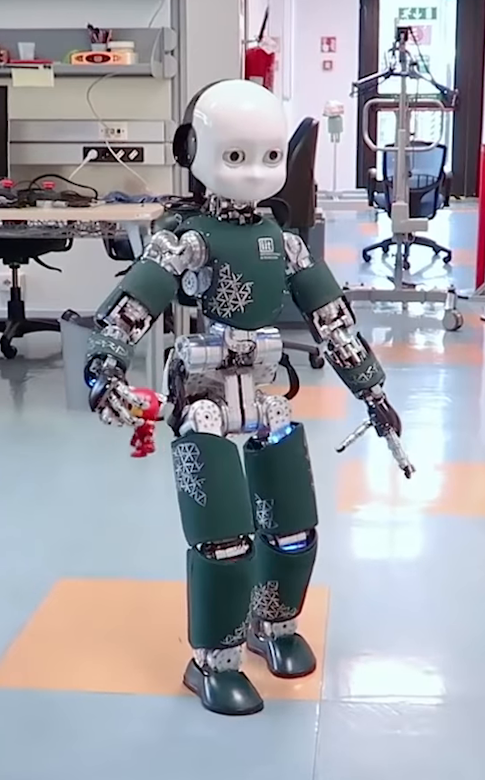
\includegraphics[width=\columnwidth]{chapter_simplified_benchmarking/figures/step1.png}
    \end{subfigure}
    \hfill
           \begin{subfigure}[b]{0.32\textwidth}
        \centering
        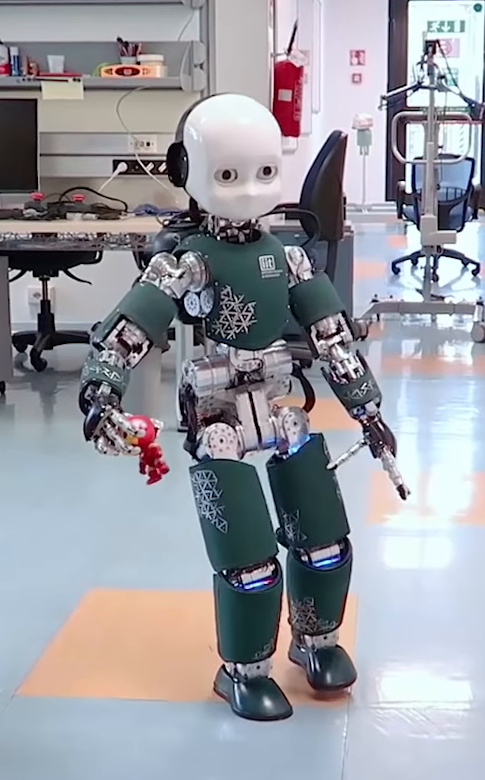
\includegraphics[width=\columnwidth]{chapter_simplified_benchmarking/figures/step2.png}
    \end{subfigure}
    \hfill
           \begin{subfigure}[b]{0.32\textwidth}
        \centering
        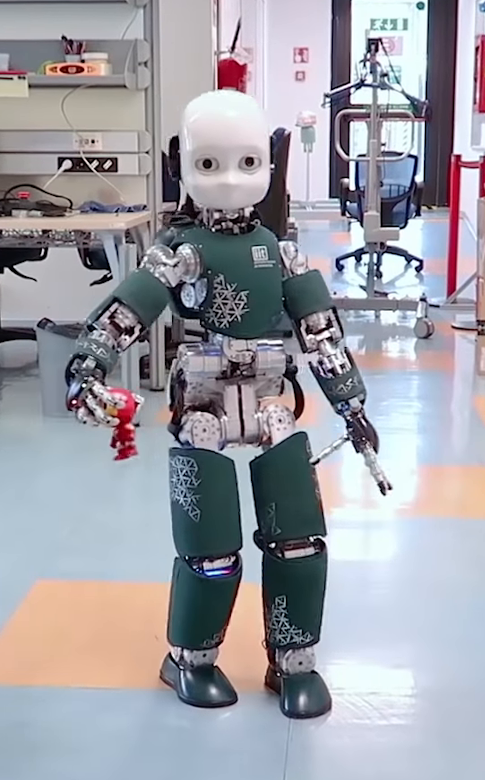
\includegraphics[width=\columnwidth]{chapter_simplified_benchmarking/figures/step3.png}
    \end{subfigure}
    \caption{The iCub robot walks with the 3 layer controller architecture of Figure~\ref{fig:three-layer-simplified-benchmarking}.}
    \label{fig:icub_walking_simplified}
\end{figure}

\section{Results}
\label{sec:results_simplified_benchmarking}
In this section, we present experiments obtained with several implementations of the simplified model controllers, namely: the \emph{instantaneous} and the \emph{predictive} controllers.

To benchmark the different simplified model controllers, we test the algorithms on the iCub humanoid robot v2.7 -- Section~\ref{sec:icub2.7}. We attach the simplified control layer to the three-layer controller architecture shown in Figure~\ref{fig:three-layer}. In this framework, the whole-body control layer implements the kinematics-based whole-body QP presented in section~\ref{sec:ik_qp}. Figure~\ref{fig:icub_walking_simplified} shows the humanoid robot iCub walking with the simplified models controller presented in this chapter.

The control architecture runs on the iCub head's computer, namely a 4-th generation Intel \textsuperscript{\tiny\textregistered} Core i7 @ $\SI{1.7}{\giga \hertz}$. In any of its implementations, the architecture takes (on average) less than $\SI{3}{\milli \second}$ to evaluate its output. The code is open source completely developed in C++: \href{https://github.com/robotology/walking-controllers}{\texttt{https://github.com/robotology/walking-controllers}}. The MPC problem presented in Section~\ref{predictive-control} is solved using the OSQP~\citep{Stellato2018} library~\footnote{Since our code is  written in pure C++, the QP problem is written by means of \texttt{osqp-eigen} a C++ wrapper for OSQP \href{https://github.com/robotology/osqp-eigen}{\texttt{https://github.com/robotology/osqp-eigen}}}.


Table~\ref{tab:max_velocity} summarizes the maximum velocities achieved using the different implementations of the control architecture. In particular, the labels \emph{instantaneous} and \emph{predictive} mean that the associated layer generates its output considering inputs and references either at the single time $t$ or for a time window, respectively. The labels, \emph{velocity} and \emph{position} control, instead, mean that the layer outputs are either desired joint velocities or position, respectively -- see Section~\ref{subsubsec-pos-vel-control}. 

\begin{table}[b]
    \centering
    \caption{Maximum forward straight walking velocities achieved using different implementations of the control architecture.
    }
    \begin{tabular}{cc|c}
         \begin{tabular}{@{}c@{}}Simplified Model  Control\end{tabular} &
         \begin{tabular}{@{}c@{}}Whole-Body QP Control\end{tabular} &
         \begin{tabular}{@{}c@{}}Max Straight Velocity (m/s)\end{tabular}\\
        \hline
        Predictive  & Velocity  &  0.1563\\
        Predictive  & Position  & 0.1645\\
        Instantaneous  & Velocity  &  0.1809\\
        Instantaneous  & Position  & 0.3372
    \end{tabular}
    \label{tab:max_velocity}
\end{table}

Let us remark that all the implemented control architectures exploit the controller presented in Section~\ref{ZMP-CoM-Controller} to attempt the stabilization of the desired center of pressure and desired center of mass position and velocity. The performance of this controller is highly dependent on the gains $K_{zmp}$ and $K_{com}$. In particular, we observed that the gains in achieving good tracking during standing and walking were not the same. For this reason, we implemented a gain-scheduling technique depending on whether the robot is walking or standing. The transition between the two sets of gains is smoothed with a minimum jerk trajectory \citep{Pattacini2010}.


To compare the simplified models controllers, we decided to perform two main experiments. These two experiments represent the maximum robot velocity that has been achieved with all architectures and the maximum velocity achieved with a specific architecture only -- see Table~\ref{tab:max_velocity}. That is, 
\begin{itemize}
    \item[-] \textbf{Experiment 1}: a forward robot speed of $\SI{0.1563}{\meter \per \second}$;
    \item[-] \textbf{Experiment 2}: a forward robot speed of $\SI{0.3372}{\meter \per \second}$.
\end{itemize}

\begin{figure}[t]
    \centering
    \begin{myframe}{Instantaneous + Position Control}
        \centering
    \begin{subfigure}[b]{0.49\textwidth}
        \centering
        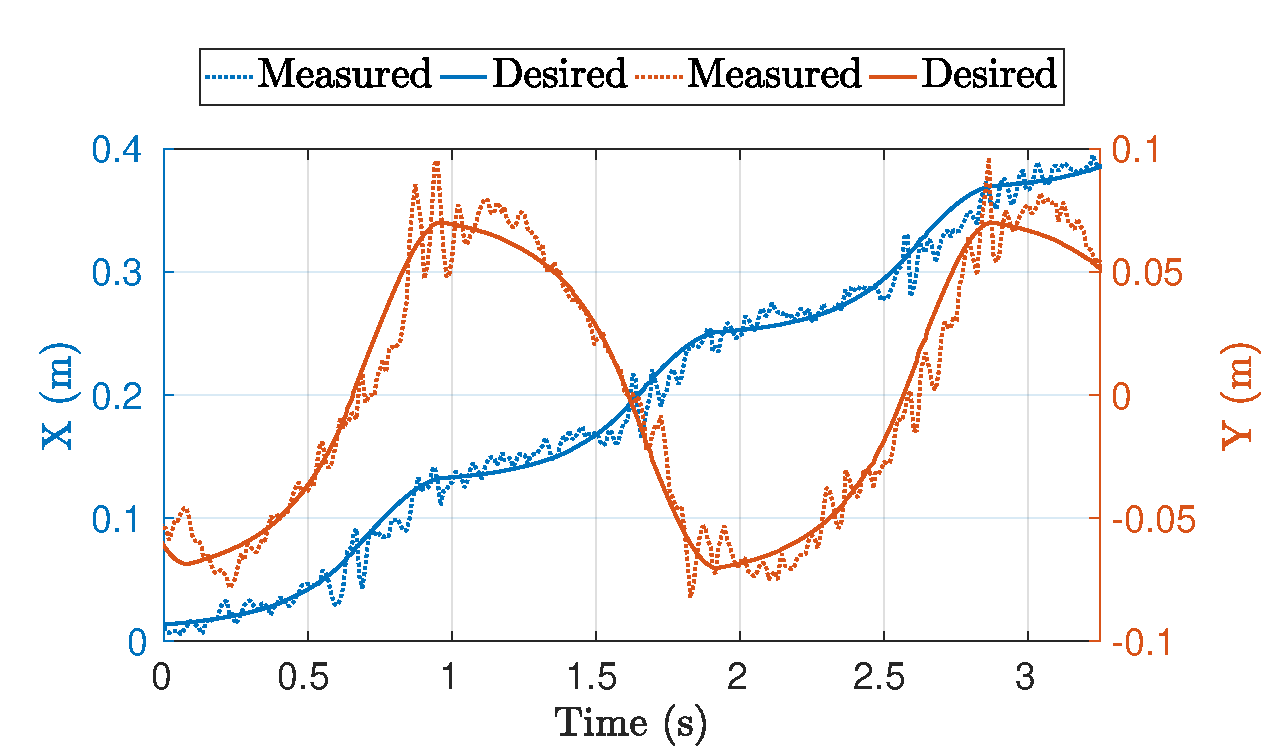
\includegraphics[width=\textwidth]{chapter_simplified_benchmarking/figures/inst_pos-min_vel-dcm.pdf}
        \caption{DCM}
        \label{fig:inst_pos-min_vel-dcm}
    \end{subfigure}
    \hfill
    \begin{subfigure}[b]{0.49\textwidth}
        \centering
        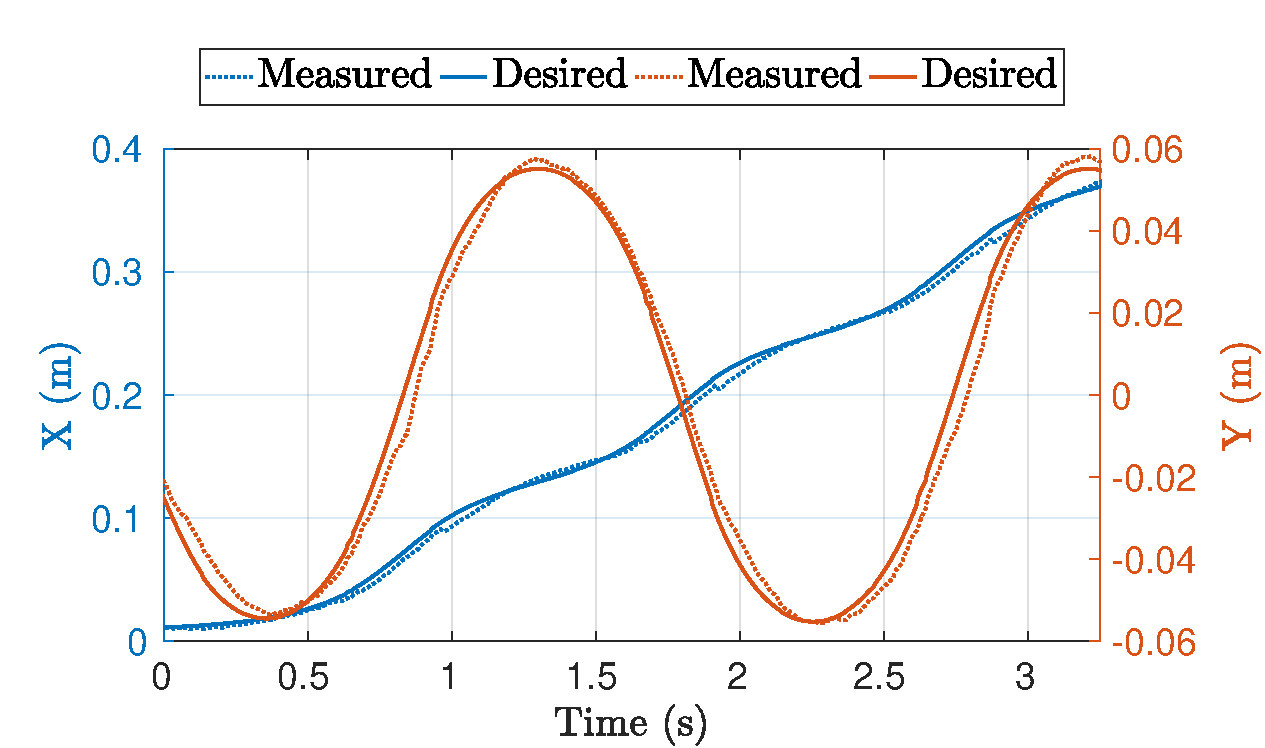
\includegraphics[width=\textwidth]{chapter_simplified_benchmarking/figures/inst_pos-min_vel-com.pdf}
        \caption{CoM}
        \label{fig:inst_pos-min_vel-com}
    \end{subfigure}
    \hfill
    \begin{subfigure}[b]{0.49\textwidth}
        \centering
        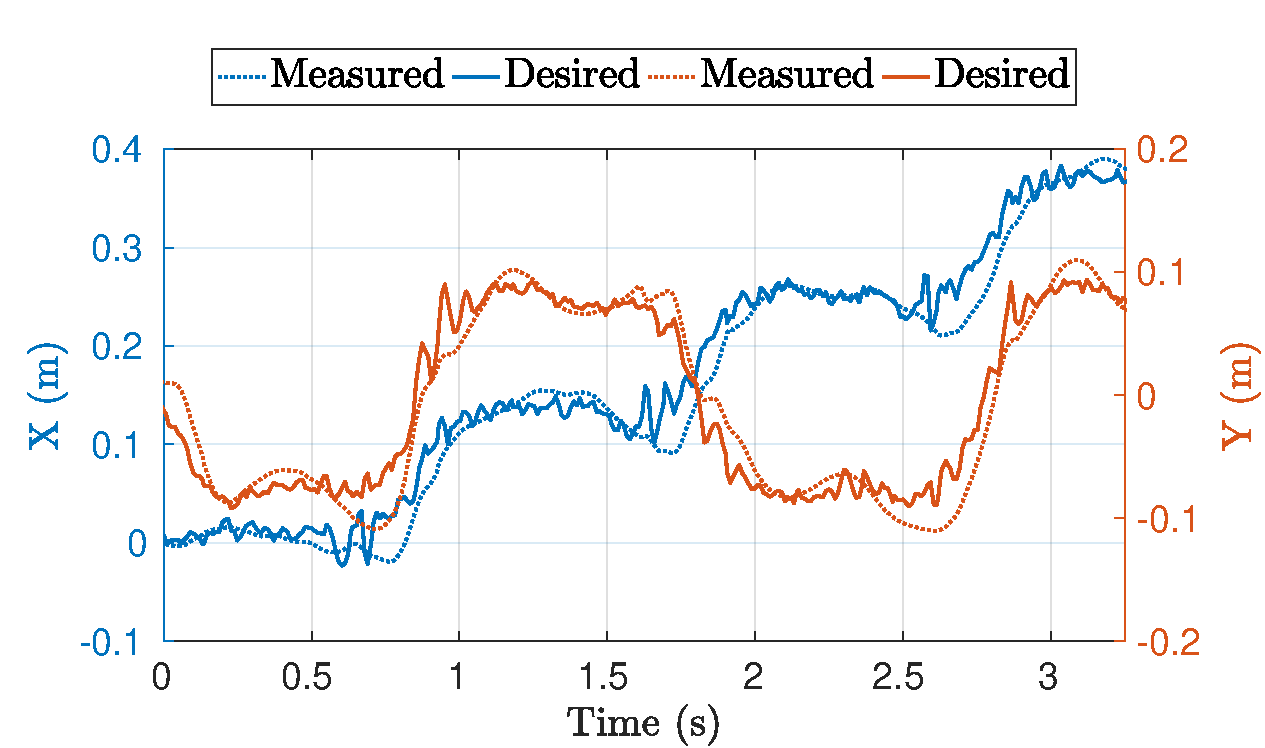
\includegraphics[width=\textwidth]{chapter_simplified_benchmarking/figures/inst_pos-min_vel-zmp.pdf}
        \caption{ZMP}
        \label{fig:inst_pos-min_vel-zmp}
    \end{subfigure}
    \end{myframe}
    \caption{Tracking of the DCM (a), CoM (b) and ZMP (c) using the instantaneous controller with the whole-body controller as position control. Walking velocity:  $\SI{0.19}{\meter \per \second}$.}
\end{figure}

\begin{figure}[t]
    \begin{myframe}{Predictive + Position Control}
     \centering
    \begin{subfigure}[b]{0.49\textwidth}
        \centering
        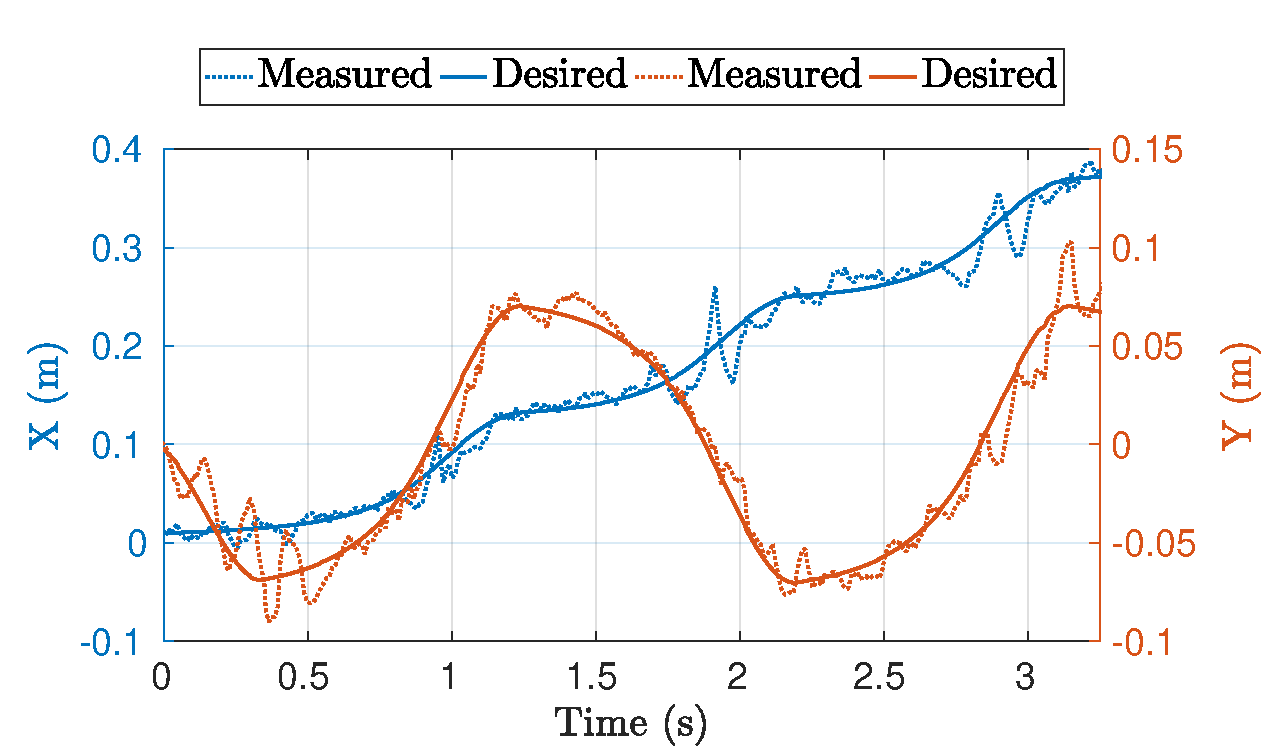
\includegraphics[width=\textwidth]{chapter_simplified_benchmarking/figures/mpc_pos-min_vel-dcm.pdf}
        \caption{DCM}
        \label{fig:mpc_pos-min_vel-dcm}
    \end{subfigure}
    \hfill
    \begin{subfigure}[b]{0.49\textwidth}
        \centering
        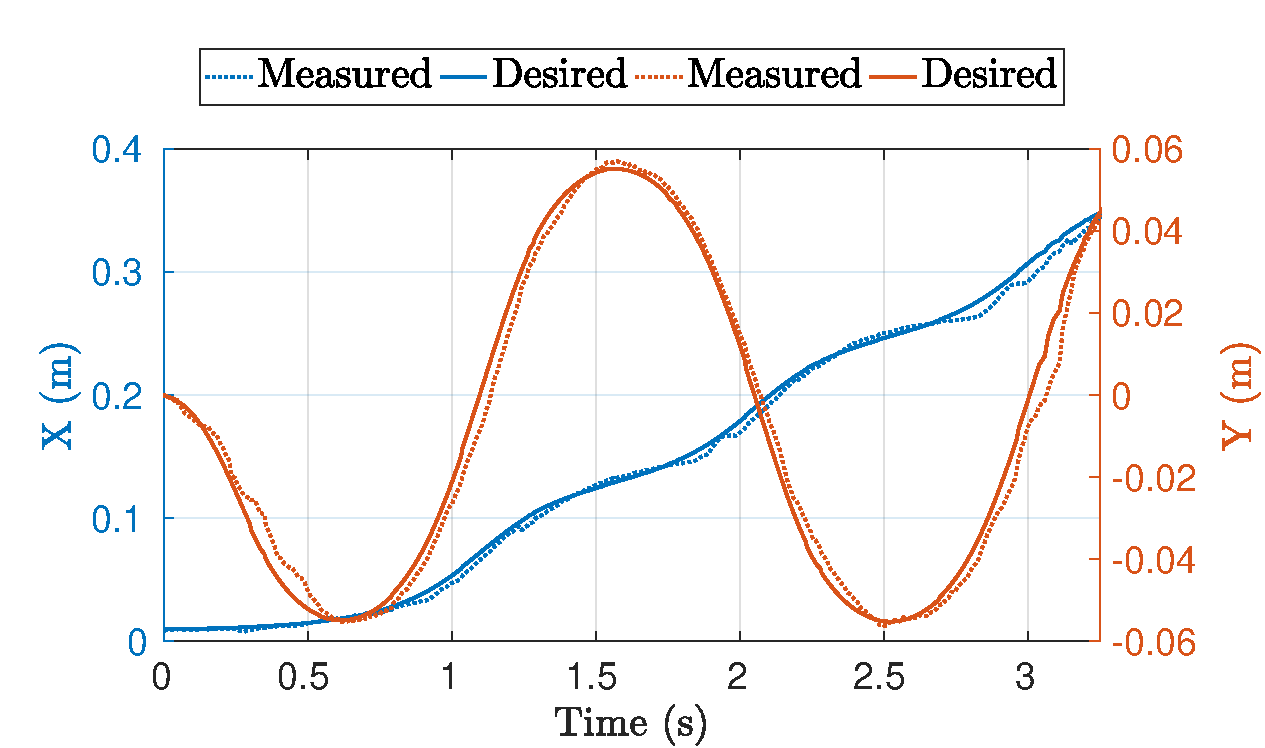
\includegraphics[width=\textwidth]{chapter_simplified_benchmarking/figures/mpc_pos-min_vel-com.pdf}
        \caption{CoM}
        \label{fig:mpc_pos-min_vel-com}
    \end{subfigure}
         \begin{subfigure}[b]{0.49\textwidth}
        \centering
        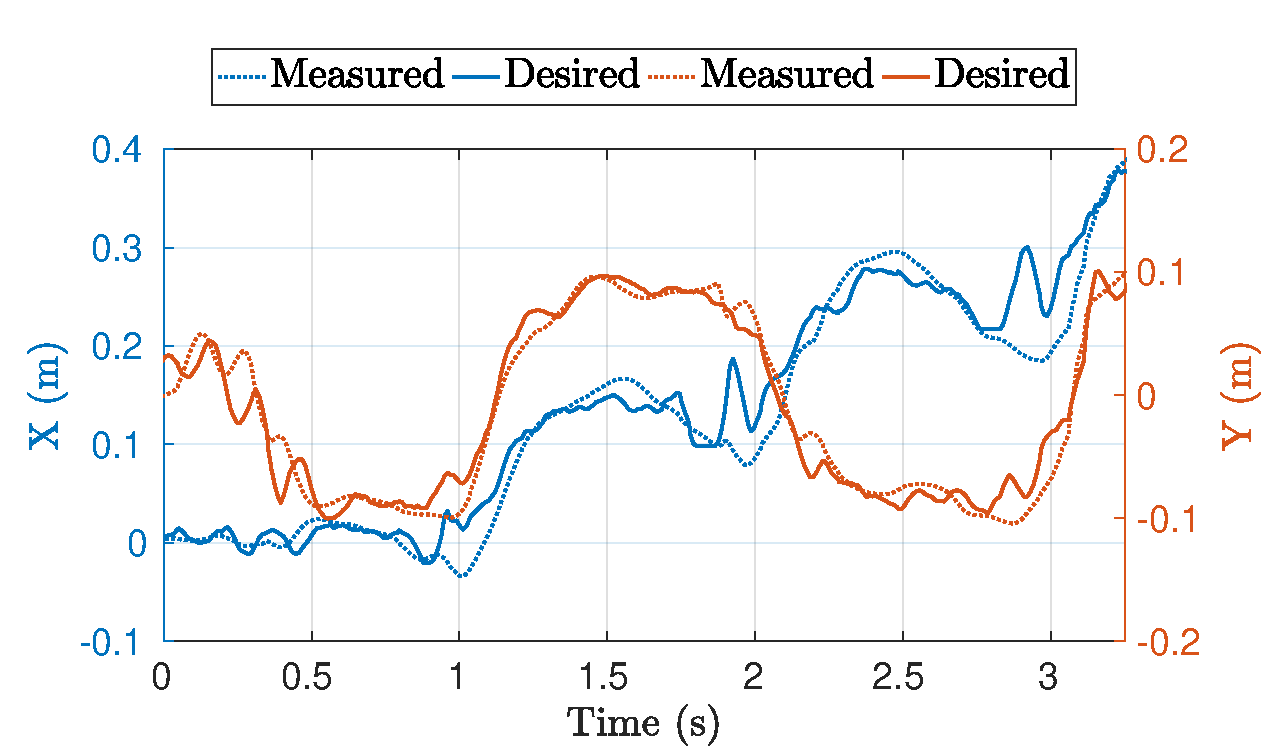
\includegraphics[width=\textwidth]{chapter_simplified_benchmarking/figures/mpc_pos-min_vel-zmp.pdf}
        \caption{ZMP}
        \label{fig:mpc_pos-min_vel-zmp}
    \end{subfigure}
    \end{myframe}
    \caption{Tracking of the  DCM (a), CoM (b) and ZMP (c) using the MPC and the whole-body controller as position control. Walking velocity:  $\SI{0.19}{\meter \per \second}$.}
\end{figure}
\begin{figure}[t]
     \vspace*{-0.1cm}
    \begin{myframe}{Instantaneous + Position Control}
    \centering
        \begin{subfigure}[b]{0.49\textwidth}
        \centering
        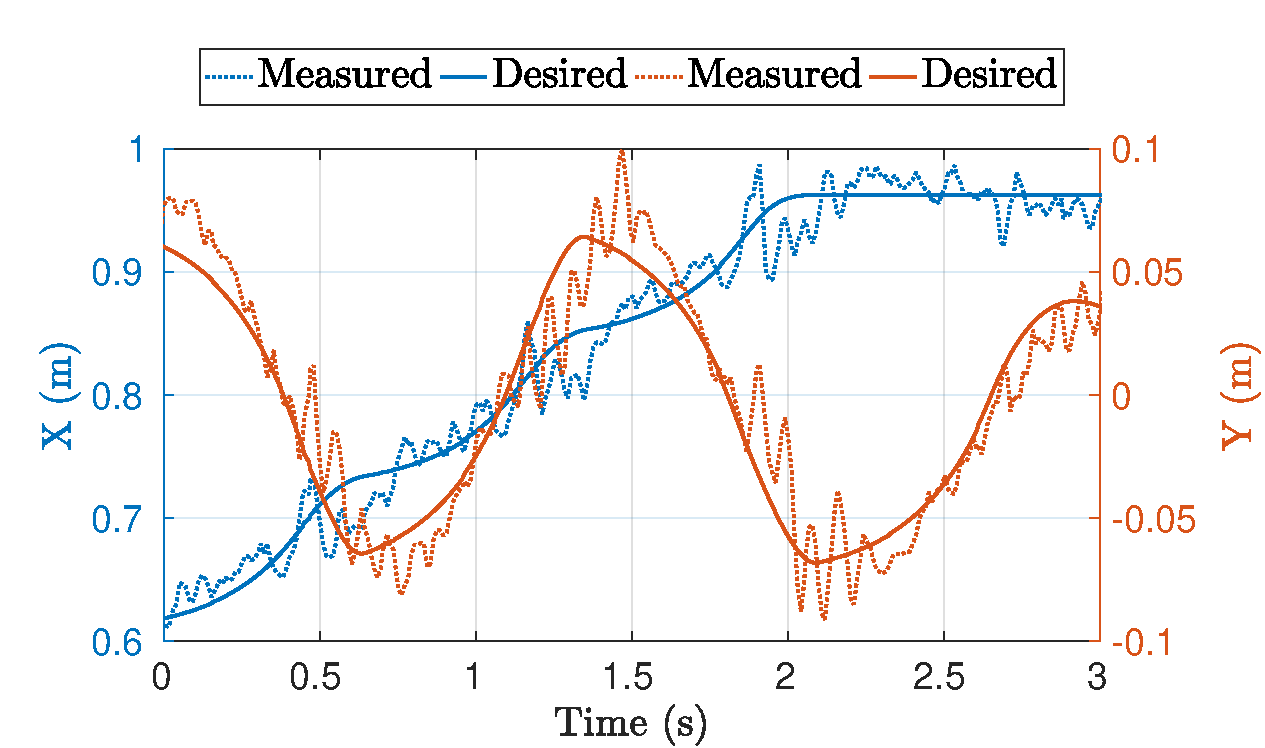
\includegraphics[width=\textwidth]{chapter_simplified_benchmarking/figures/inst_pos-max_vel-dcm.pdf}
        \caption{DCM}
        \label{fig:inst_pos-max_vel-dcm}
    \end{subfigure}
    \hfill
     \begin{subfigure}[b]{0.49\textwidth}
        \centering
        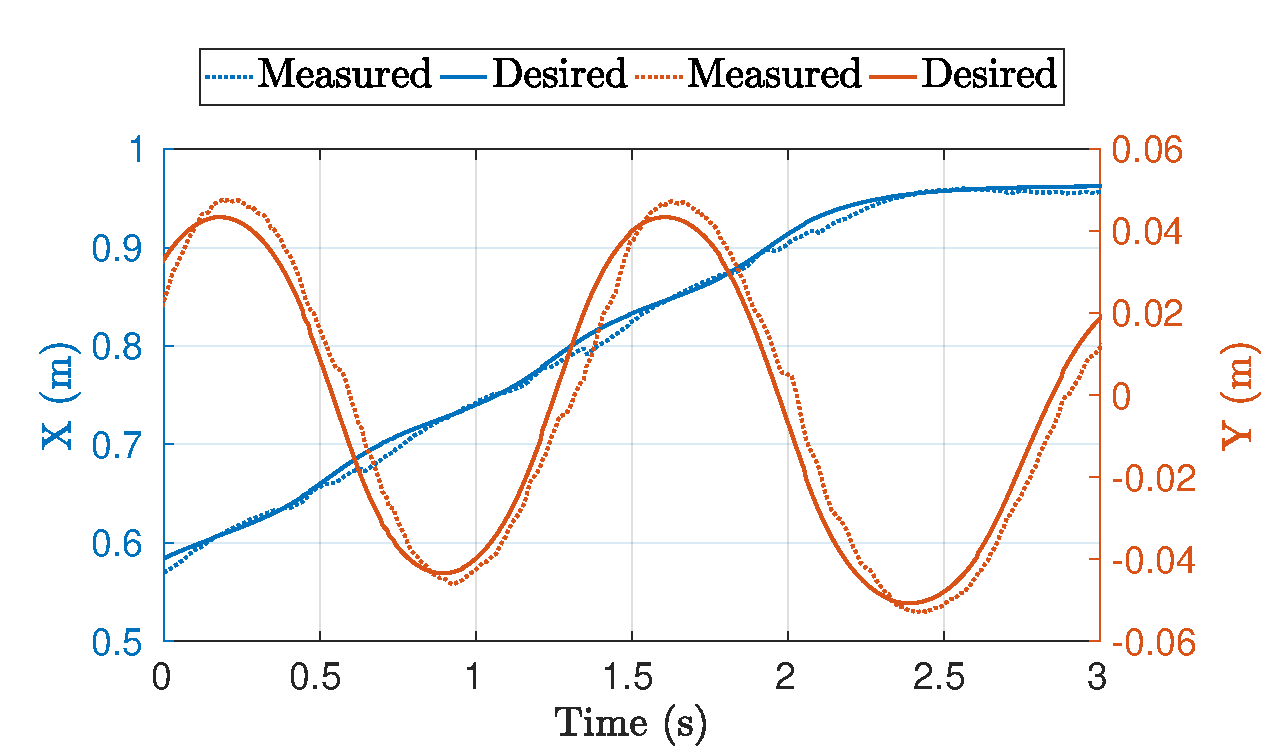
\includegraphics[width=\textwidth]{chapter_simplified_benchmarking/figures/inst_pos-max_vel-com.pdf}
        \caption{CoM}
        \label{fig:inst_pos-max_vel-com}
    \end{subfigure}
    \hfill
    \begin{subfigure}[b]{0.49\textwidth}
        \centering
        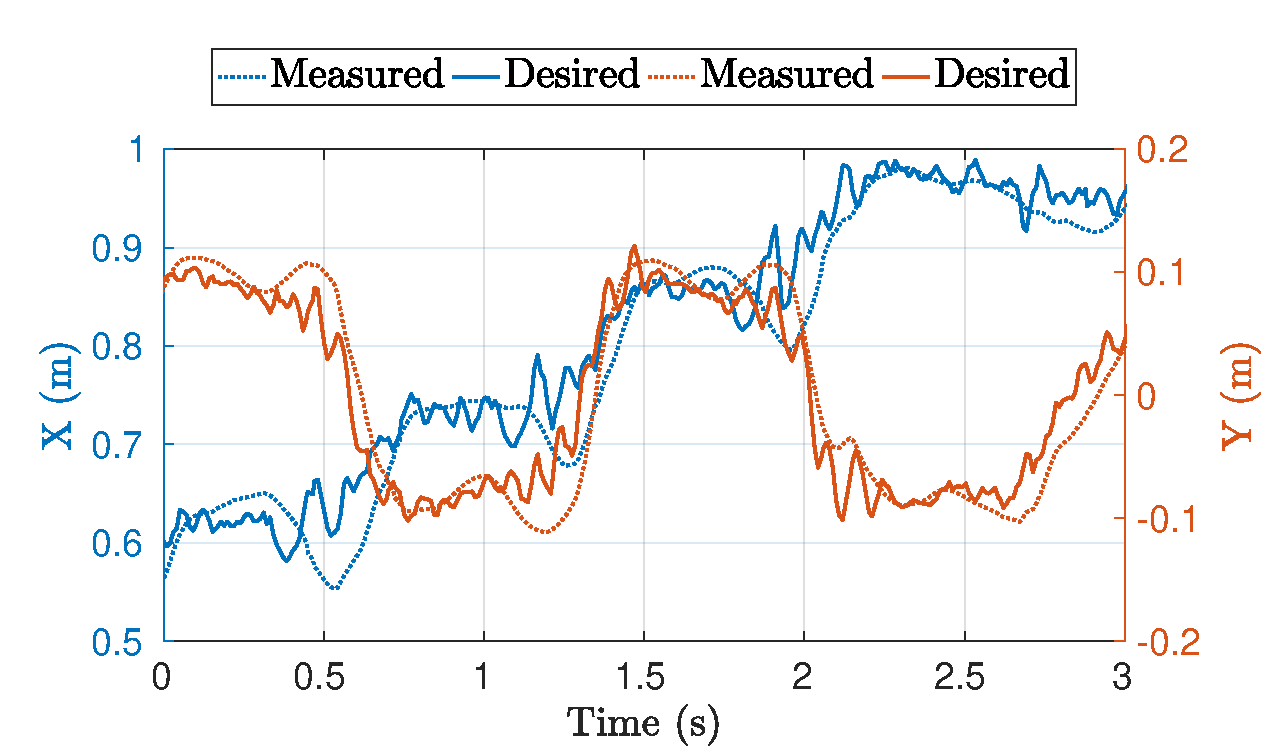
\includegraphics[width=\textwidth]{chapter_simplified_benchmarking/figures/inst_pos-max_vel-zmp.pdf}
        \caption{ZMP}
        \label{fig:inst_pos-max_vel-zmp}
    \end{subfigure}
    \end{myframe}
    \caption{Tracking of the DCM (a), CoM (b) and ZMP (c) with the instantaneous and whole-body QP control as position.  Walking velocity: $\SI{0.41}{\meter \per \second}$.}
\end{figure}
\begin{figure}[t]
    \begin{myframe}{Predictive + Position Control}
    \centering
    \begin{subfigure}[b]{0.49\textwidth}
        \centering
        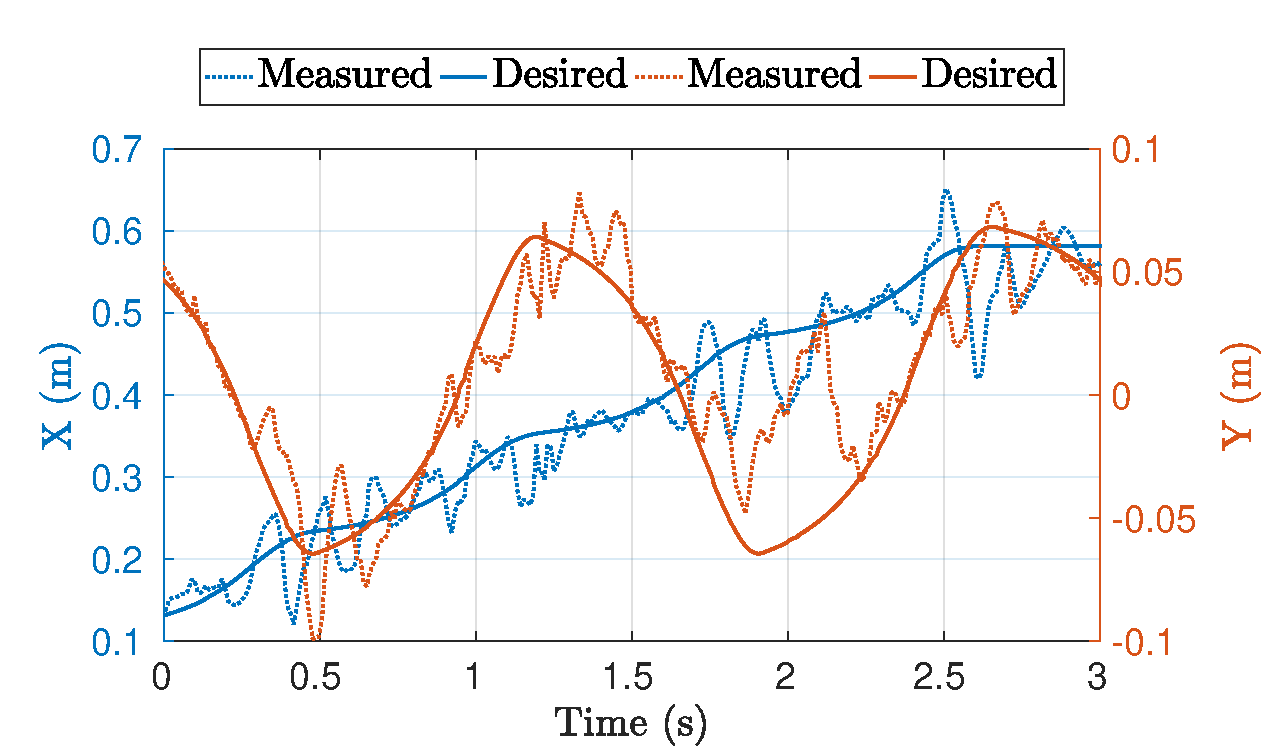
\includegraphics[width=\textwidth]{chapter_simplified_benchmarking/figures/mpc_pos-max_vel-dcm.pdf}
        \caption{DCM}
        \label{fig:mpc_pos-max_vel-dcm}
    \end{subfigure}
    \hfill
     \begin{subfigure}[b]{0.49\textwidth}
        \centering
        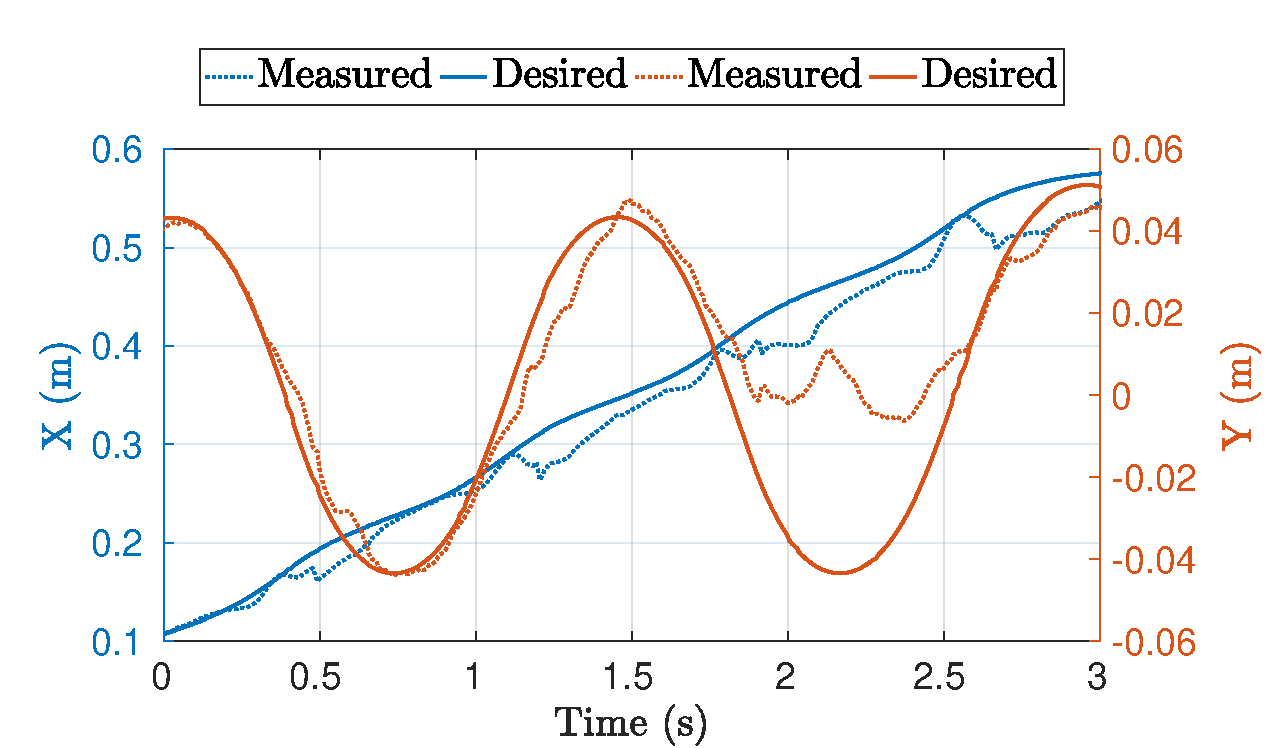
\includegraphics[width=\textwidth]{chapter_simplified_benchmarking/figures/mpc_pos-max_vel-com.pdf}
        \caption{CoM}
        \label{fig:mpc_pos-max_vel-com}
    \end{subfigure}
    \hfill
    \begin{subfigure}[b]{0.49\textwidth}
        \centering
        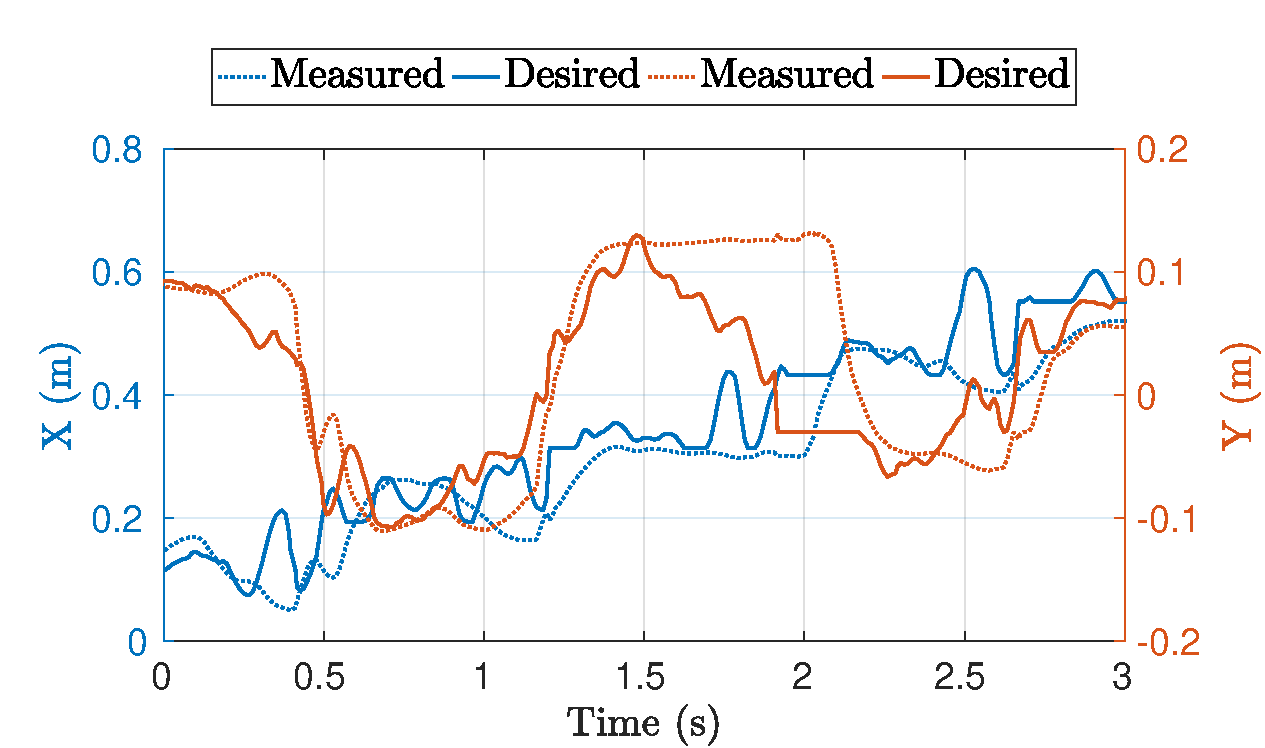
\includegraphics[width=\textwidth]{chapter_simplified_benchmarking/figures/mpc_pos-max_vel-zmp.pdf}
        \caption{ZMP}
        \label{fig:mpc_pos-max_vel-zmp}
    \end{subfigure}
    \end{myframe}
    \caption{Tracking of the  DCM (a), CoM (b) and ZMP (c) with the predictive and whole-body QP control as position control. At $t\approx \SI{2}{\second}$, the robot falls down.  Walking velocity: $\SI{0.41}{\meter \per \second}$.}
    \vskip-0.5cm
\end{figure}

We compare the control laws~\eqref{eq:reactive_dcm} and~\eqref{eq:mpc_solution_simplified}, which both generate a (desired) center of pressure that attempts to stabilize the desired DCM. To simplify the comparison, the controller of the \emph{whole-body QP layer} is kept fixed in this section, and we show and discuss only the results when the robot is position controlled. A complete comparison of the kinematics-based whole-body controllers is presented in Section~\ref{sec:wbc_experimental_results}.
In the following experiments, we set the time horizon of the predictive control to $\SI{2}{\second}$.

\subsection{Experiment 1: a forward robot speed of 0.1563 m s$^{\text{-1}}$}
Figures \ref{fig:inst_pos-min_vel-dcm} and \ref{fig:mpc_pos-min_vel-dcm} show the DCM tracking performances obtained with the instantaneous and predictive controllers, respectively. Both controllers seem to show good tracking performances, and the DCM error is kept below $\SI{5}{\centi \meter}$ in both cases. Note, however, that the instantaneous controller induces faster variations of the measured DCM. This contributes to the overall higher vibrations of the robot. One of the reasons for this variation is that the instantaneous controller~\eqref{eq:reactive_dcm} injects a (desired) center of pressure proportional to the measured DCM, which in turn contains the center of mass velocity. To mitigate this, we may filter the joint velocities appropriately. However, in our case, the joint velocities were not filtered to avoid delays in the measured DCM. Our experience showed that adding a filter to joint velocities is not an easy task, and we did not find the right trade-off for obtaining overall performance improvements. 

Figures~\ref{fig:inst_pos-min_vel-com} and \ref{fig:mpc_pos-min_vel-com} present CoM tracking performances, which are mainly dependent on the ZMP-CoM controller~\eqref{eq:ZMP_controller}. This controller receives the desired DCM values from the \emph{simplified model control} layer, which are obtained with the instantaneous or predictive controllers. In both cases, the CoM error is kept below $\SI{2}{\centi \meter}$. Figures~\ref{fig:inst_pos-min_vel-zmp} and~\ref{fig:mpc_pos-min_vel-zmp} represent the ZMP tracking performance, which is still mainly dependent on the ZMP-CoM controller~\eqref{eq:ZMP_controller}. It is important to note that the desired ZMP is smoother when the \emph{simplified model control} uses the predictive law~\eqref{eq:mpc_solution_simplified} to generate it. Indeed, this is a tunable property that depends on the associated weight in the cost function of the MPC problem. Although this smoother behavior contributes to less robot vibrations, overall robot performance became less reactive and, consequently, less robust to robot falls. Although the extensive hand-made tuning, we were not able to increase the robot velocity when the \emph{simplified model control} used the predictive law~\eqref{eq:mpc_solution_simplified}. 

\subsection{Experiment 2: a forward robot speed of 0.3372 m s$^{\text{-1}}$}
At a robot's desired walking speed of $\SI{0.3372}{\meter \per \second}$, there is initially no significant difference between the DCM tracking obtained with instantaneous and predictive control laws -- see Figures~\ref{fig:mpc_pos-max_vel-dcm} and~\ref{fig:inst_pos-max_vel-dcm} for $t < \SI{1.5}{\second}$. However, fast robot walking velocities require fast variations of the desired CoM and ZMP. This fast variation degrades the performance of the predictive controller around $t = \SI{1.5}{\second}$ -- see Figure~\ref{fig:mpc_pos-max_vel-zmp}. Clearly, these bad performances, in turn, induce poor tracking of the DCM shown in Figure~\ref{fig:mpc_pos-max_vel-dcm} at $t\approx \SI{2}{\second}$, and consequently the robot falls. At this point, one is tempted to increase the gain $K_\text{ZMP}$ of the controller~\eqref{eq:ZMP_controller}, which shall induce a better tracking of the ZMP. Unfortunately, this leads to higher robot oscillations induced by the noise on the estimated ZMP. And, as a consequence, the robot falls. 

We can conclude that the \emph{predictive simplified control} is much less robust than the \emph{instantaneous simplified control} with respect to ZMP tracking errors. Adding a low-pass filter to the ZMP measurement may improve the overall performance. However, in our case, adding filters led to slower system response and, consequently, to the robot falling.



\section{Conclusions \label{sec:conclusions_flexible_joint}}
This chapter presents the design of a whole-body QP control layer for a humanoid robot affected by link flexibility. We model the flexibility by introducing equivalent passive joints that simulate the motion caused by the link deformation.
We then considered the passive joints position and velocity as state of the floating base system dynamics. Thanks to this choice, we develop a whole-body controller that implicitly considers the joint flexibility in the stabilization problem. 
The chapter also details the design of an estimator that aims at computing the flexible joint state in real-time. 
\par
The proposed approach is validated in a simulated version of the TALOS humanoid robot, where its hip flexibility has a significant impact while performing locomotion tasks. Moreover, the architecture is then compared with a whole-body controller that considers all links of the robot rigid.
\par
As a future work, we plan to mitigate the discontinuity of the contact forces by performing a smother transition between contiguous support phases. We also plan to make a detailed comparison with other state-of-the-art controllers that
consider the flexibility of the robot link~\citep{Villa2022TorqueFlexibility}. In addition, we plan to validate the architecture on the real robot.



